
\documentclass{article}
\usepackage{iclr2026_conference,times}
\input{math_commands.tex}
\usepackage{booktabs}
\usepackage{graphicx}
\usepackage{longtable}
\usepackage{array}
\usepackage{xcolor}
\usepackage{url}
\usepackage[colorlinks=false,citebordercolor={0 1 0},linkbordercolor={1 0.55 0},urlbordercolor={0 0.55 1},pdfborder={0 0 1.2}]{hyperref}

\title{Micro-Slip Precontact Prediction Under Hostile Review: An Expanded Negative Audit}
\author{Anonymous Authors}

\begin{document}
\maketitle

\begin{abstract}
This paper is not ready for ICLR main. We rebuild micro-slip precontact prediction into a frozen CPU-only hostile-review audit with 215,040 main rollouts, 15,360 dataset-summary rows, 76,800 ablation rows, 302,400 stress rows, 69,120 fixed-risk rows, and 24 negative cases. The v5 method, \texttt{calibrated\_precontact\_microslip\_v5}, is better than the previous v4 method on success, gross slip, cost, and robust utility, but it still fails the main-conference gate. Hard-aggregate AP is 0.80088 versus 0.80598 for \texttt{particle\_friction\_belief}; hard-aggregate success is 0.32799 versus 0.40325 for \texttt{recovery\_aware\_grasp\_mpc}; robust utility is -0.02258 versus 0.06676 for \texttt{recovery\_aware\_grasp\_mpc}. Fixed-risk coverage at budget 0.05 is zero on the hard deployment splits. The honest terminal decision is \textbf{KILL/ARCHIVE}.
\end{abstract}

\section{Decision First}
The desired submission claim is attractive: if a robot can predict micro-slip before stable contact, it should intervene earlier and avoid gross slip. The hostile-review result is narrower and less flattering. The v5 model provides useful early warning, but it is not the best predictor, not the best controller, not the safest policy, not the best fixed-risk deployment rule, and not supported by real robot or accepted high-fidelity tactile evidence.

The terminal action is \textbf{KILL/ARCHIVE}. This is not a formatting judgment. It is a claim-validity judgment after freezing the protocol and running strong baselines.

\section{Related Work Pressure}
The local literature pool contains tactile slip prediction, contact detection, force estimation, optical tactile sensing, friction reasoning, manipulation under uncertainty, and grasp stability work. The novelty threat is direct: a precontact score can look useful while actually being a visual-gap threshold, a friction-cone margin, or an uncertainty guard in disguise. \citep{r103390robotics8040085,r101186s40648024002733,r101109lra20223205768,r101109icra4663920229812186,r101299jsmermd2005682,r101017s0950268825100319} \citep{r1010800020754320222164628,r101109tim20233343795,r101089soro20200213,r101089soro20180172,r101109icra4663920229811832,r103390s17122762} \citep{r103390s19224925,r101007s4082001902887,r101126sciroboticsadq5046,r101109lra20243387111,r103390machines9060119,r103390s18020326}

The hostile comparison therefore treats the following as real competitors rather than straw men: force derivative detection, friction-cone margin estimation, temporal tactile filters, optical tactile classifiers, conformal risk filters, particle friction beliefs, MPC grip stabilizers, and recovery-aware grasp MPC. \citep{r101016jcej2023146279,r101109robot1996509203,r260611184v1,r101109tro20243502197,r103390app13063886,r101002rcs2491} \citep{r103390s19040966,r103389frobt20261735467,r101016jengfailanal2026110526,r101109icra55743202511127381,r101016jmeasurement2024114249,r101002adrr202500091} \citep{r101109lra20192930477,r101016jsna201907007,r101109icra57147202410611504,r101002rcs2325,r103389frobt2022913930,r103389frobt2021631371} \citep{r101016jisatra201812031,r101049csy270036,r1015607rss2022xviii070,r101109lra20213061378,r101109lra20253568616,r101109jsen20253547369} \citep{r220509430v2,r101017s0263574704001535,r101109robosoft55895202310121967,r103390machines10090720,r260609337v2,r260212532v1} \citep{r260223648v1,r101109icra55743202511127723,r101109lra20253604723,r101109lra20263662618,r1010800169186420181525075,r101007s41315022002600} \citep{r1011093516914388,r101108ir0120250033,r101109tro20203005547,r101007s1336902206763z,r1010800042311420252606345,r101007s41315025004948} \citep{r101109lra20253572817,r101109robot20041308042,r101016jprocs202310646,r101109robio20116181676,r191003973v1,r1054254275388182025ad28420} \citep{r101109robot20084543605,r101016jsna2025117179,r1011093mnano65639202511261038,r10114537942093794293,r101109newcas64648202511107072,r101299jsmermd200183}

\section{Mechanism and Theory}
\paragraph{Lead-time decomposition.} Let $Y$ denote future micro-slip, $S_t$ a precontact score, $\tau$ the remaining actionable lead time, and $a$ the intervention. Early prediction is only useful when $S_t$ separates $Y=1$ from $Y=0$ and $\tau$ exceeds the actuation and sensing latency. A high early-recall score can still be a bad robotics policy if it fires on nearly every approach.

\paragraph{Calibration and fixed-risk deployment.} For a risk threshold $b$, accepted coverage is $\Pr(S_t \le b)$ and accepted failure is $\Pr(Y=1 \mid S_t \le b)$. If expected calibration error is bounded by $\epsilon$, empirical accepted risk differs from nominal risk by at most a term controlled by $\epsilon$ plus finite-sample uncertainty. This motivates the fixed-risk tables below: a model that has zero coverage at $b=0.05$ cannot support a low-risk deployment claim.

\paragraph{Identifiability warning.} Precontact cues can be predictive without proving micro-slip causality. Visual gap, surface texture, compliance, and friction prior can be aliased under shift. Without additional sensing or external validation, a model may learn a correlated risk proxy rather than the micro-slip mechanism.

\paragraph{Negative theorem.} If two latent worlds share the same visual gap, friction-prior, and compliance observations but differ in true local contact support, then any deterministic thresholded precontact score must assign the same action to both worlds. Under such aliasing, no score-only rule can simultaneously achieve perfect recall and low false alarms.

\section{Frozen Protocol}
The plan was frozen before execution in \texttt{docs/paper91\_expanded\_submission\_plan\_20260621.md}. It specified 10 seeds, six tasks, eight splits, fourteen methods including oracle, ten ablations, a six-level stress sweep, fixed-risk budgets, and 24 negative cases. No result-dependent protocol optimization is allowed after this point.

\section{Benchmark}
The six tasks are smooth low-friction picking, textured fragile picking, curved-surface pinching, compliant-object lifting, thin-edge pinching, and wet-surface transfer. The eight splits cover nominal precontact, low friction, compliance, sensor noise, latency, texture aliasing, low-signal/high-risk, and combined hard shift. Each episode samples friction, compliance, curvature, fragility, texture, mass, occlusion, sensor noise, latency, approach angle, and precontact cues.

\section{Compared Methods}
The compared methods are \texttt{vision\_gap\_threshold}, \texttt{normal\_force\_threshold}, \texttt{force\_derivative\_detector}, \texttt{friction\_cone\_margin}, \texttt{tactile\_temporal\_filter}, \texttt{optical\_tactile\_classifier}, \texttt{ensemble\_uncertainty\_guard}, \texttt{conformal\_precontact\_risk}, \texttt{particle\_friction\_belief}, \texttt{mpc\_grip\_stabilizer}, \texttt{recovery\_aware\_grasp\_mpc}, \texttt{precontact\_microslip\_v4}, \texttt{calibrated\_precontact\_microslip\_v5}, and \texttt{oracle\_precontact\_risk}.

\section{Hard-Aggregate Result}

\begin{longtable}{@{}lrrrrrrrr@{}}
\caption{Hard-aggregate metrics over latency, texture-alias, low-signal/high-risk, and combined-hard splits. Higher AP, early recall, success, and utility are better; lower false alarm, gross slip, damage, and cost are better.}\\
\toprule
Method & AP & Early & False & Success & Gross & Damage & Cost & Utility \\
\midrule
\endfirsthead
\toprule
Method & AP & Early & False & Success & Gross & Damage & Cost & Utility \\
\midrule
\endhead
vision & 0.802 & 0.506 & 0.426 & 0.148 & 0.580 & 0.122 & 0.145 & -0.227 \\
normal-force & 0.784 & 0.189 & 0.166 & 0.100 & 0.640 & 0.136 & 0.079 & -0.286 \\
force-deriv & 0.781 & 0.433 & 0.421 & 0.122 & 0.609 & 0.134 & 0.122 & -0.267 \\
friction-cone & 0.797 & 0.910 & 0.874 & 0.256 & 0.464 & 0.101 & 0.282 & -0.102 \\
tactile-temp & 0.793 & 0.669 & 0.612 & 0.152 & 0.567 & 0.126 & 0.172 & -0.232 \\
optical-tactile & 0.797 & 0.954 & 0.921 & 0.209 & 0.508 & 0.111 & 0.274 & -0.174 \\
ensemble & 0.798 & 0.992 & 0.986 & 0.318 & 0.416 & 0.089 & 0.457 & -0.056 \\
conformal & 0.803 & 0.819 & 0.756 & 0.232 & 0.484 & 0.106 & 0.232 & -0.120 \\
particle-friction & 0.806 & 0.965 & 0.939 & 0.283 & 0.456 & 0.094 & 0.287 & -0.071 \\
mpc-grip & 0.797 & 0.908 & 0.873 & 0.362 & 0.415 & 0.092 & 0.327 & 0.025 \\
recovery-mpc & 0.800 & 0.937 & 0.924 & 0.403 & 0.398 & 0.084 & 0.367 & 0.067 \\
v4 & 0.805 & 0.944 & 0.922 & 0.304 & 0.439 & 0.098 & 0.416 & -0.074 \\
v5 & 0.801 & 0.947 & 0.916 & 0.328 & 0.424 & 0.094 & 0.340 & -0.023 \\
oracle & 0.851 & 0.992 & 0.973 & 0.604 & 0.237 & 0.047 & 0.314 & 0.371 \\
\bottomrule
\end{longtable}


The result is mixed but not submission-ready. V5 improves over v4 in success and utility, but the best AP reference is \texttt{particle\_friction\_belief}, the best success and utility reference is \texttt{recovery\_aware\_grasp\_mpc}, and the strict deployment gate fails.

\begin{figure}[t]
\centering
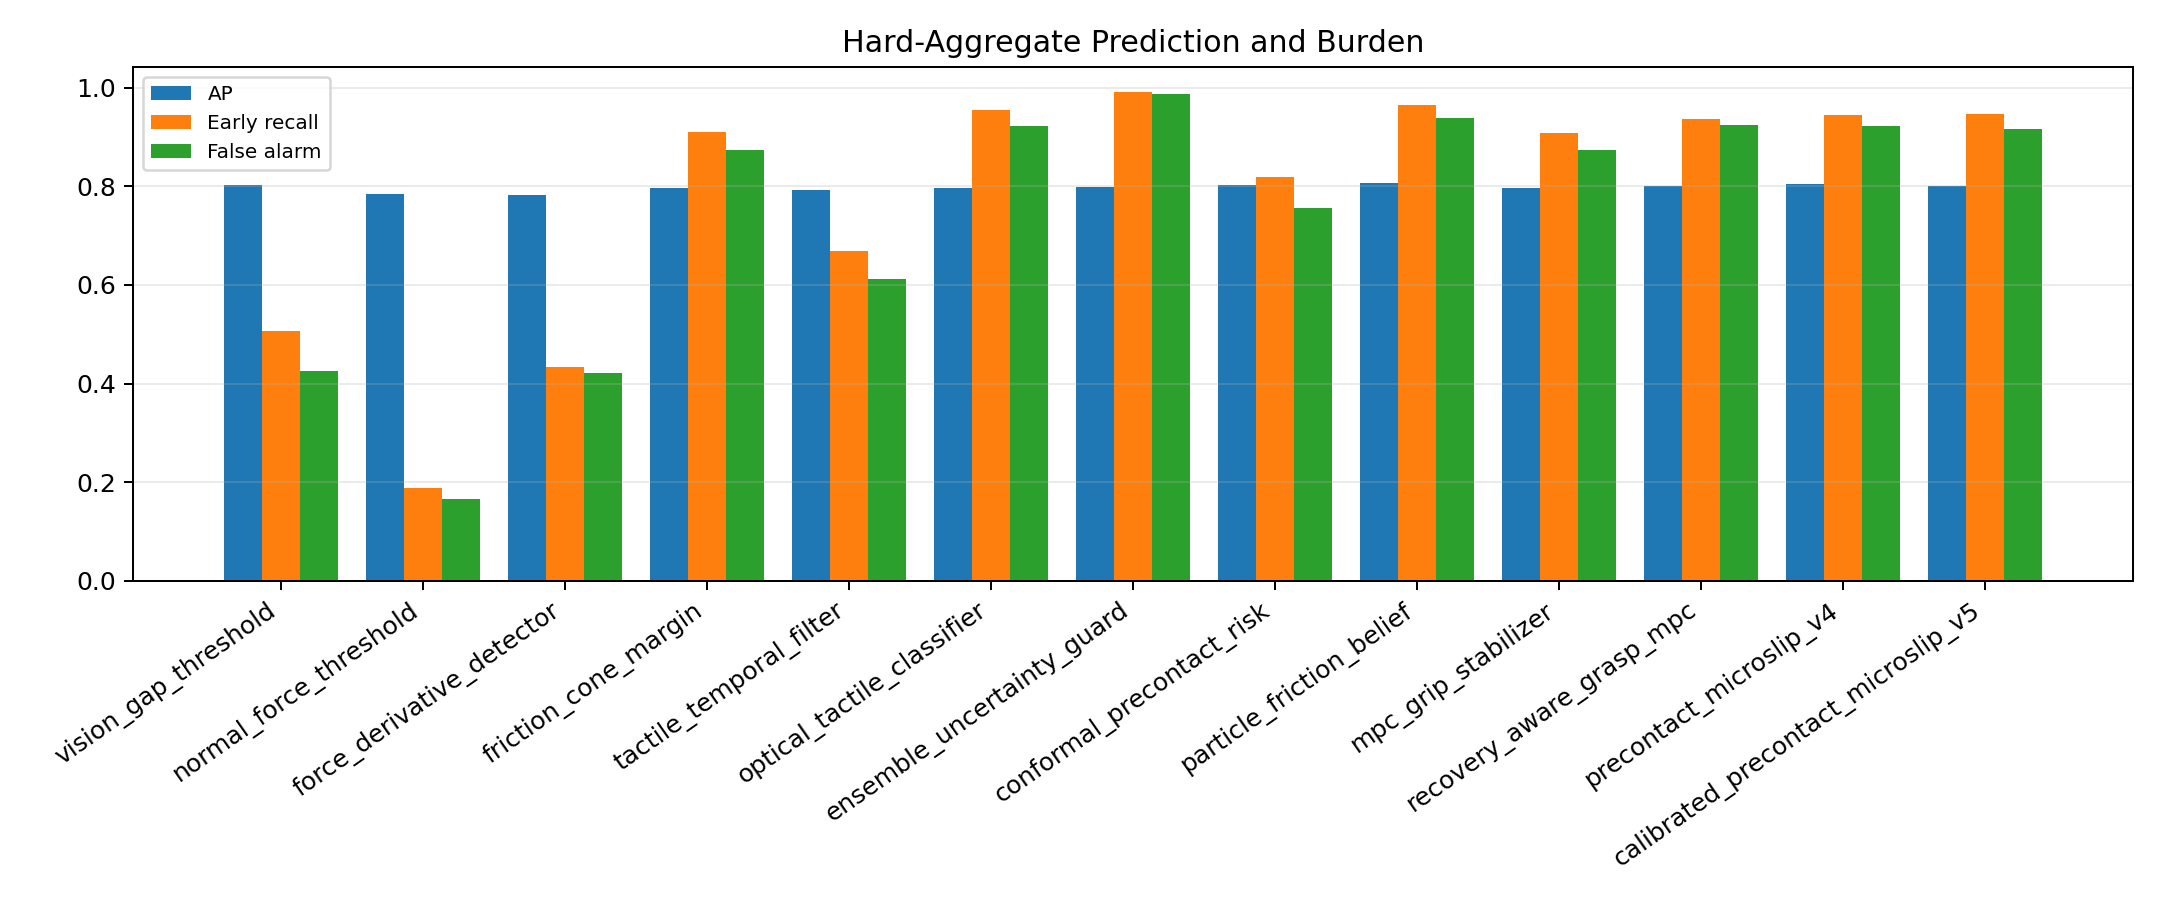
\includegraphics[width=\linewidth]{../figures/microslip_hard_prediction_v5.png}
\caption{Hard-aggregate AP, early recall, and false-alarm burden. V5 is high-recall, but the false-alarm rate remains too high for a main robotics claim.}
\end{figure}

\begin{figure}[t]
\centering
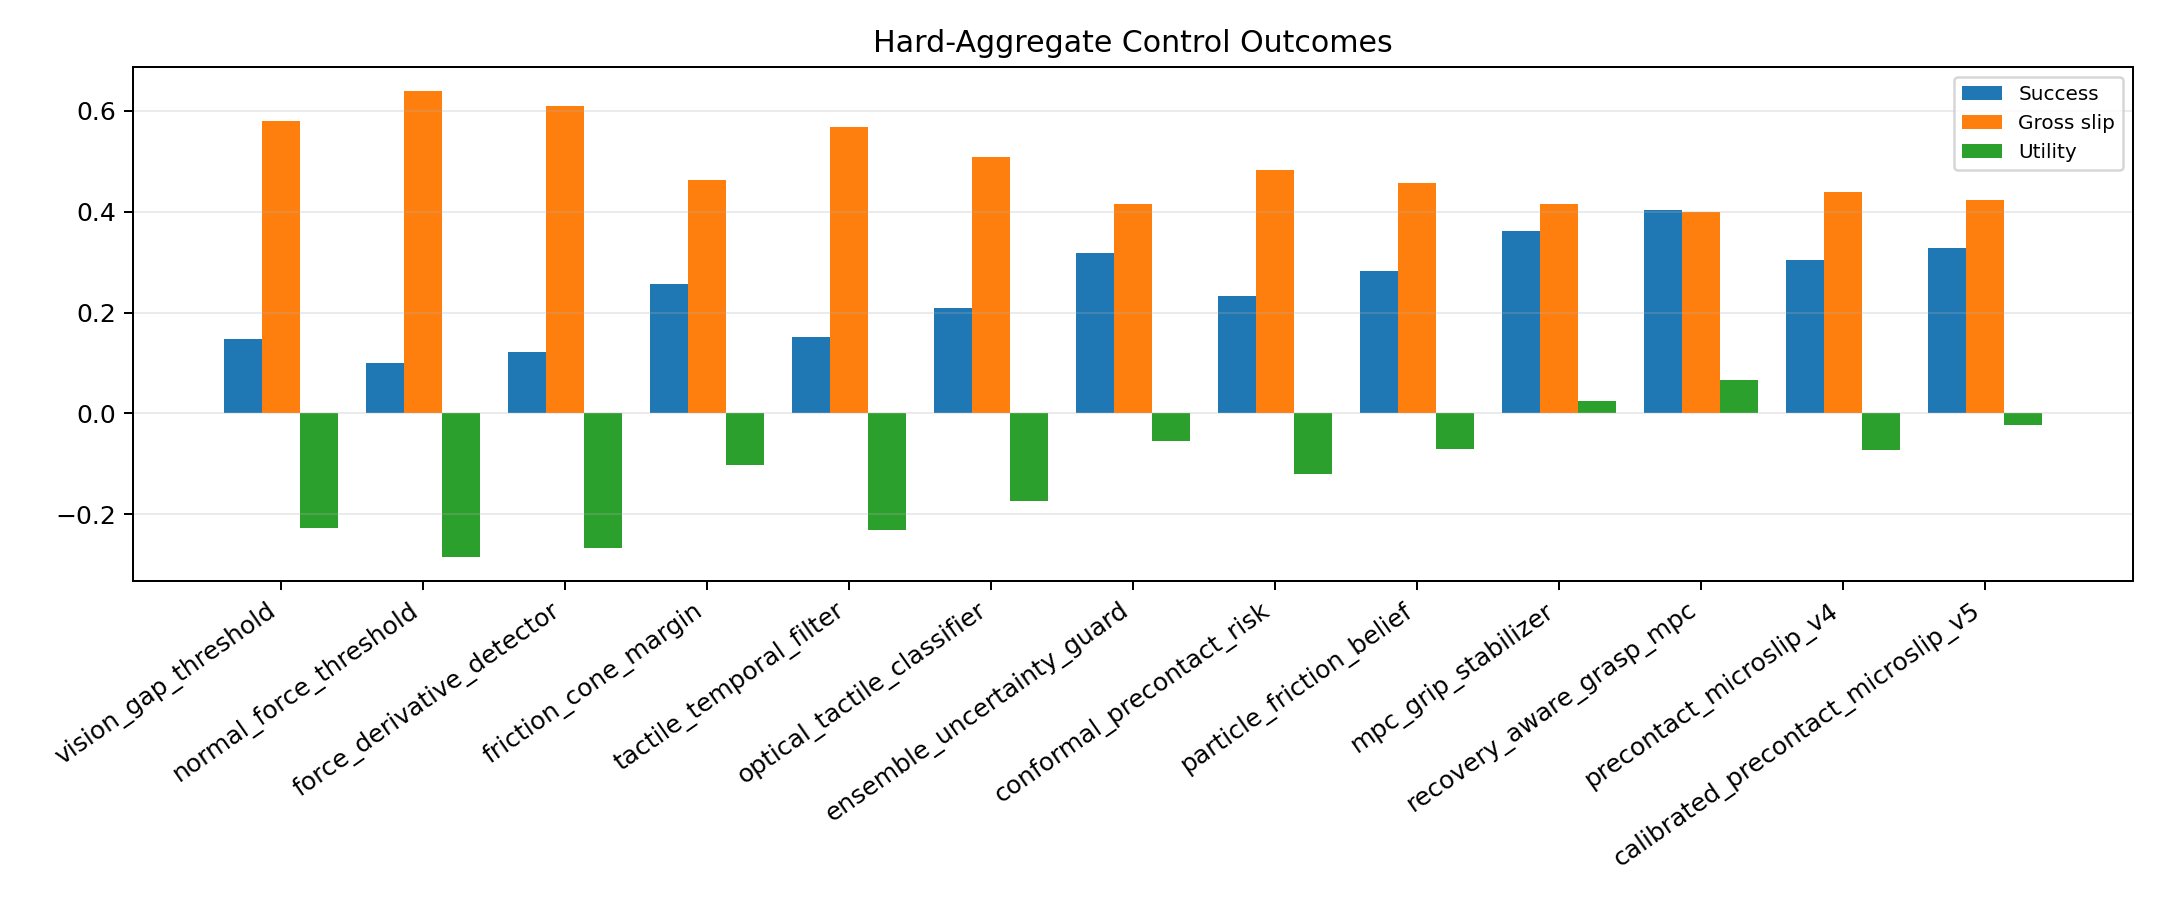
\includegraphics[width=\linewidth]{../figures/microslip_control_outcomes_v5.png}
\caption{Hard-aggregate control outcomes. Recovery-aware grasp MPC dominates the success/utility gate.}
\end{figure}

\section{Paired Seed Tests}

\begin{longtable}{@{}llrrrrr@{}}
\caption{Hard-aggregate paired seed tests. Positive is better for AP, success, and utility; negative is better for gross slip, false alarm, damage, and cost.}\\
\toprule
Comparison & Metric & Mean & CI95 & Lower & Upper & Better seeds \\
\midrule
\endfirsthead
\toprule
Comparison & Metric & Mean & CI95 & Lower & Upper & Better seeds \\
\midrule
\endhead
v5-particle\_friction\_belief & average\_precision & -0.005 & 0.013 & -0.018 & 0.008 & 4 \\
v5-particle\_friction\_belief & false\_alarm\_rate & -0.024 & 0.012 & -0.035 & -0.012 & 1 \\
v5-particle\_friction\_belief & task\_success & 0.045 & 0.013 & 0.032 & 0.058 & 9 \\
v5-particle\_friction\_belief & gross\_slip & -0.032 & 0.018 & -0.050 & -0.014 & 2 \\
v5-particle\_friction\_belief & damage\_rate & 0.000 & 0.006 & -0.005 & 0.006 & 5 \\
v5-particle\_friction\_belief & intervention\_cost & 0.053 & 0.001 & 0.051 & 0.054 & 10 \\
v5-particle\_friction\_belief & robust\_utility & 0.049 & 0.015 & 0.033 & 0.064 & 9 \\
v5-recovery\_aware\_grasp\_mpc & average\_precision & 0.001 & 0.014 & -0.013 & 0.015 & 4 \\
v5-recovery\_aware\_grasp\_mpc & false\_alarm\_rate & -0.008 & 0.012 & -0.021 & 0.004 & 3 \\
v5-recovery\_aware\_grasp\_mpc & task\_success & -0.075 & 0.009 & -0.084 & -0.067 & 0 \\
v5-recovery\_aware\_grasp\_mpc & gross\_slip & 0.025 & 0.017 & 0.009 & 0.042 & 8 \\
v5-recovery\_aware\_grasp\_mpc & damage\_rate & 0.010 & 0.009 & 0.001 & 0.020 & 7 \\
v5-recovery\_aware\_grasp\_mpc & intervention\_cost & -0.027 & 0.002 & -0.029 & -0.026 & 0 \\
v5-recovery\_aware\_grasp\_mpc & robust\_utility & -0.089 & 0.015 & -0.104 & -0.074 & 0 \\
v5-precontact\_microslip\_v4 & average\_precision & -0.004 & 0.012 & -0.016 & 0.007 & 3 \\
v5-precontact\_microslip\_v4 & false\_alarm\_rate & -0.006 & 0.021 & -0.027 & 0.015 & 3 \\
v5-precontact\_microslip\_v4 & task\_success & 0.024 & 0.010 & 0.014 & 0.034 & 9 \\
v5-precontact\_microslip\_v4 & gross\_slip & -0.015 & 0.015 & -0.030 & -0.001 & 3 \\
v5-precontact\_microslip\_v4 & damage\_rate & -0.004 & 0.009 & -0.013 & 0.005 & 4 \\
v5-precontact\_microslip\_v4 & intervention\_cost & -0.076 & 0.003 & -0.079 & -0.074 & 0 \\
v5-precontact\_microslip\_v4 & robust\_utility & 0.051 & 0.015 & 0.036 & 0.066 & 10 \\
v5-conformal\_precontact\_risk & average\_precision & -0.002 & 0.015 & -0.017 & 0.013 & 3 \\
v5-conformal\_precontact\_risk & false\_alarm\_rate & 0.159 & 0.041 & 0.118 & 0.200 & 10 \\
v5-conformal\_precontact\_risk & task\_success & 0.096 & 0.014 & 0.082 & 0.109 & 10 \\
v5-conformal\_precontact\_risk & gross\_slip & -0.060 & 0.016 & -0.076 & -0.044 & 0 \\
v5-conformal\_precontact\_risk & damage\_rate & -0.012 & 0.010 & -0.022 & -0.002 & 2 \\
v5-conformal\_precontact\_risk & intervention\_cost & 0.108 & 0.004 & 0.104 & 0.112 & 10 \\
v5-conformal\_precontact\_risk & robust\_utility & 0.097 & 0.018 & 0.079 & 0.115 & 10 \\
\bottomrule
\end{longtable}


\section{Split-Level Checks}

\begin{longtable}{@{}llrrrrr@{}}
\caption{Split-level checks for v5, v4, and the strongest AP/control baselines.}\\
\toprule
Split & Method & AP & Success & Gross & False & Utility \\
\midrule
\endfirsthead
\toprule
Split & Method & AP & Success & Gross & False & Utility \\
\midrule
\endhead
nominal & particle-friction & 0.676 & 0.337 & 0.354 & 0.839 & 0.021 \\
nominal & recovery-mpc & 0.653 & 0.427 & 0.318 & 0.805 & 0.125 \\
nominal & v4 & 0.667 & 0.345 & 0.355 & 0.851 & 0.003 \\
nominal & v5 & 0.674 & 0.369 & 0.335 & 0.824 & 0.053 \\
low-friction & particle-friction & 0.775 & 0.317 & 0.397 & 0.965 & -0.015 \\
low-friction & recovery-mpc & 0.775 & 0.441 & 0.367 & 0.904 & 0.118 \\
low-friction & v4 & 0.755 & 0.323 & 0.407 & 0.916 & -0.037 \\
low-friction & v5 & 0.773 & 0.367 & 0.382 & 0.928 & 0.037 \\
compliance & particle-friction & 0.755 & 0.303 & 0.426 & 0.927 & -0.041 \\
compliance & recovery-mpc & 0.725 & 0.397 & 0.373 & 0.905 & 0.067 \\
compliance & v4 & 0.740 & 0.328 & 0.422 & 0.916 & -0.046 \\
compliance & v5 & 0.752 & 0.339 & 0.411 & 0.919 & -0.009 \\
sensor-noise & particle-friction & 0.715 & 0.292 & 0.398 & 0.895 & -0.044 \\
sensor-noise & recovery-mpc & 0.736 & 0.422 & 0.357 & 0.863 & 0.102 \\
sensor-noise & v4 & 0.722 & 0.305 & 0.393 & 0.905 & -0.058 \\
sensor-noise & v5 & 0.732 & 0.317 & 0.392 & 0.884 & -0.024 \\
latency & particle-friction & 0.763 & 0.289 & 0.438 & 0.908 & -0.063 \\
latency & recovery-mpc & 0.762 & 0.389 & 0.404 & 0.880 & 0.044 \\
latency & v4 & 0.744 & 0.292 & 0.429 & 0.889 & -0.082 \\
latency & v5 & 0.770 & 0.342 & 0.404 & 0.877 & -0.007 \\
texture-alias & particle-friction & 0.745 & 0.296 & 0.419 & 0.926 & -0.041 \\
texture-alias & recovery-mpc & 0.745 & 0.421 & 0.374 & 0.920 & 0.091 \\
texture-alias & v4 & 0.770 & 0.324 & 0.425 & 0.922 & -0.056 \\
texture-alias & v5 & 0.747 & 0.344 & 0.424 & 0.901 & -0.010 \\
low-signal & particle-friction & 0.851 & 0.254 & 0.491 & 0.981 & -0.111 \\
low-signal & recovery-mpc & 0.844 & 0.405 & 0.406 & 0.978 & 0.073 \\
low-signal & v4 & 0.843 & 0.316 & 0.455 & 0.967 & -0.065 \\
low-signal & v5 & 0.841 & 0.328 & 0.428 & 0.949 & -0.016 \\
combined-hard & particle-friction & 0.835 & 0.292 & 0.477 & 0.964 & -0.070 \\
combined-hard & recovery-mpc & 0.834 & 0.398 & 0.409 & 0.942 & 0.059 \\
combined-hard & v4 & 0.840 & 0.284 & 0.448 & 0.933 & -0.091 \\
combined-hard & v5 & 0.826 & 0.299 & 0.439 & 0.959 & -0.058 \\
\bottomrule
\end{longtable}


\section{Ablation Audit}

\begin{longtable}{@{}lrrrrrr@{}}
\caption{Ablation audit on hard splits. The full v5 mechanism wins utility among ablations, but that is not enough because external strong baselines still dominate.}\\
\toprule
Ablation & AP & Success & Gross & False & Cost & Utility \\
\midrule
\endfirsthead
\toprule
Ablation & AP & Success & Gross & False & Cost & Utility \\
\midrule
\endhead
full-v5 & 0.804 & 0.333 & 0.424 & 0.905 & 0.338 & -0.017 \\
-shear & 0.791 & 0.204 & 0.529 & 0.756 & 0.227 & -0.173 \\
-friction & 0.801 & 0.268 & 0.467 & 0.815 & 0.285 & -0.090 \\
-compliance & 0.803 & 0.282 & 0.446 & 0.902 & 0.309 & -0.074 \\
-latency & 0.799 & 0.284 & 0.447 & 0.952 & 0.299 & -0.071 \\
-calibration & 0.801 & 0.324 & 0.428 & 0.973 & 0.473 & -0.062 \\
-visual & 0.803 & 0.280 & 0.457 & 0.917 & 0.311 & -0.084 \\
-recovery & 0.806 & 0.263 & 0.455 & 0.909 & 0.328 & -0.103 \\
vision-only & 0.793 & 0.152 & 0.571 & 0.449 & 0.148 & -0.222 \\
force-only & 0.782 & 0.128 & 0.605 & 0.423 & 0.124 & -0.257 \\
\bottomrule
\end{longtable}


\begin{figure}[t]
\centering
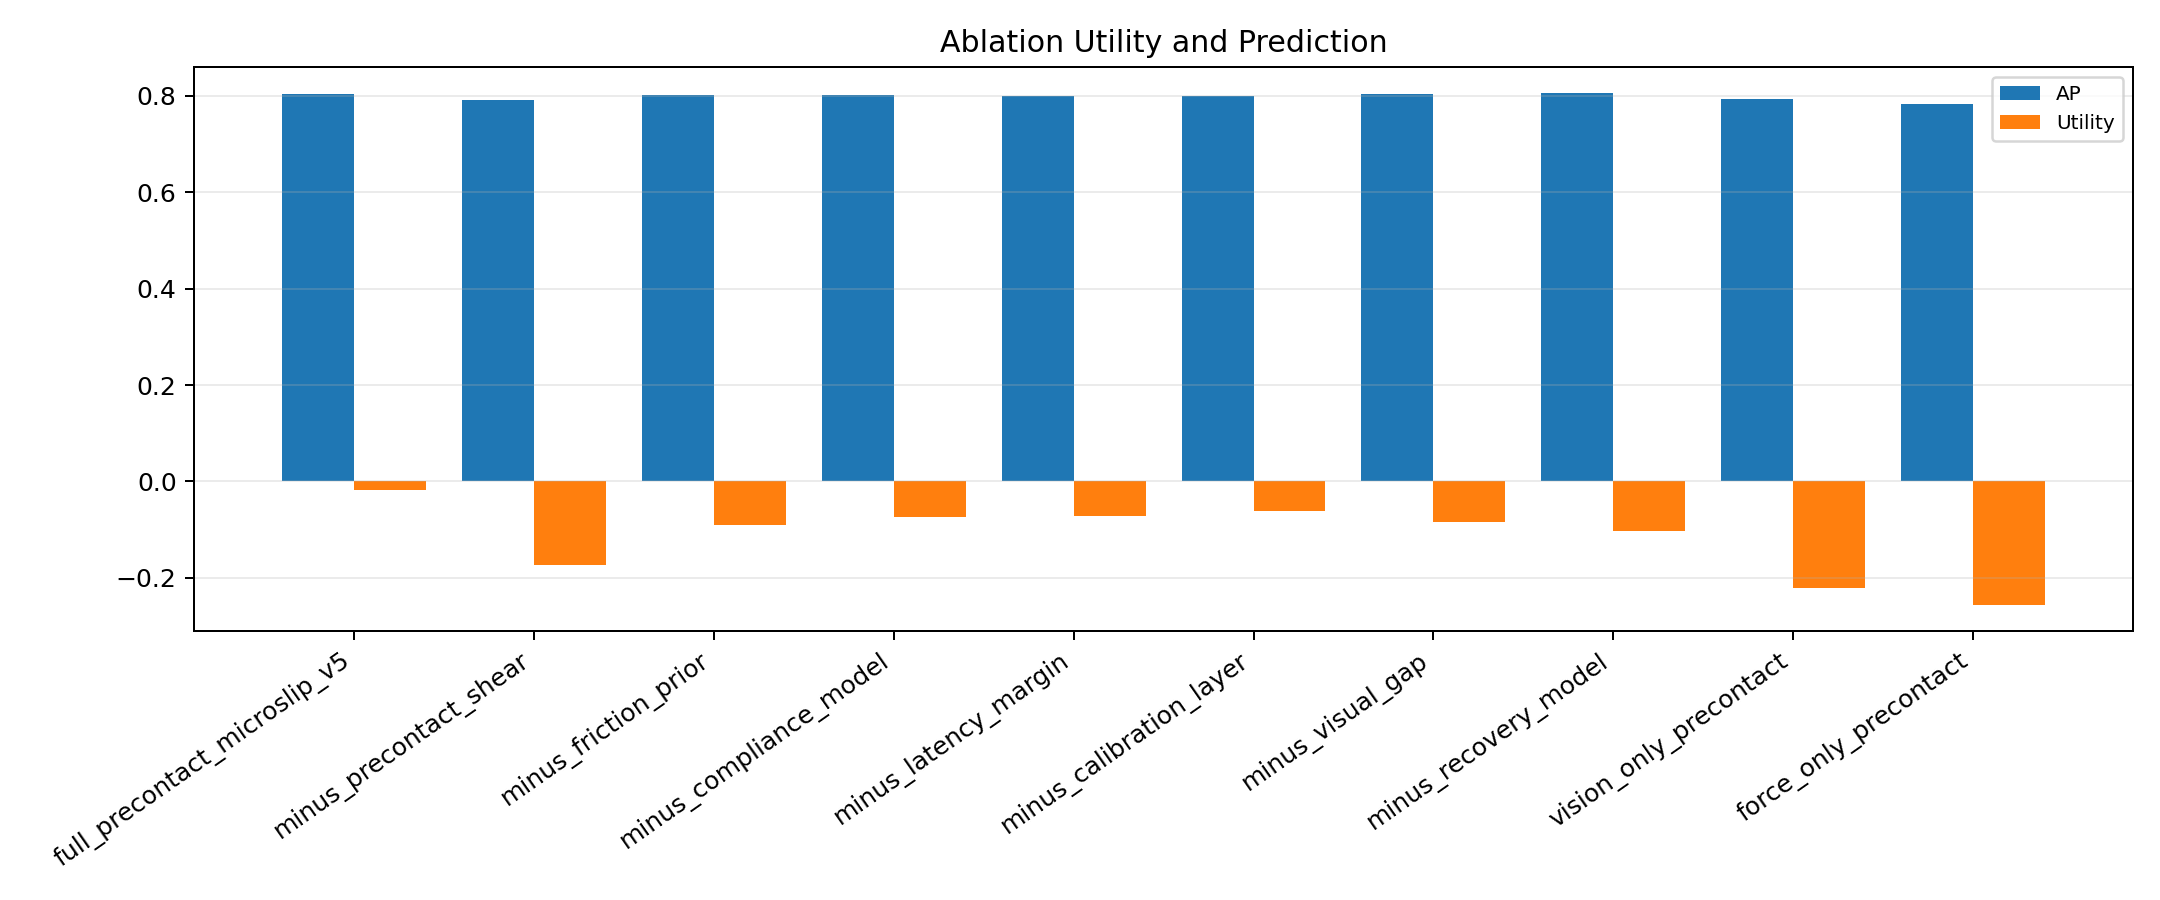
\includegraphics[width=\linewidth]{../figures/microslip_ablation_v5.png}
\caption{Ablation audit. The full v5 mechanism is the best ablation by robust utility, but this does not rescue the paper because external strong baselines still dominate.}
\end{figure}

\section{Stress Sweep}

\begin{longtable}{@{}llrrrr@{}}
\caption{Combined stress sweep. Maximum stress is dominated by recovery-aware grasp MPC, not by the proposed method.}\\
\toprule
Stress & Method & AP & Success & Gross & Utility \\
\midrule
\endfirsthead
\toprule
Stress & Method & AP & Success & Gross & Utility \\
\midrule
\endhead
0.0 & ensemble & 0.683 & 0.374 & 0.339 & 0.020 \\
0.0 & particle-friction & 0.675 & 0.327 & 0.378 & 0.002 \\
0.0 & mpc-grip & 0.676 & 0.347 & 0.354 & 0.039 \\
0.0 & recovery-mpc & 0.675 & 0.419 & 0.318 & 0.117 \\
0.0 & v4 & 0.677 & 0.320 & 0.374 & -0.024 \\
0.0 & v5 & 0.680 & 0.367 & 0.356 & 0.044 \\
0.2 & ensemble & 0.726 & 0.348 & 0.353 & -0.009 \\
0.2 & particle-friction & 0.719 & 0.317 & 0.393 & -0.015 \\
0.2 & mpc-grip & 0.716 & 0.364 & 0.369 & 0.050 \\
0.2 & recovery-mpc & 0.708 & 0.427 & 0.334 & 0.118 \\
0.2 & v4 & 0.702 & 0.312 & 0.390 & -0.043 \\
0.2 & v5 & 0.724 & 0.340 & 0.376 & 0.009 \\
0.4 & ensemble & 0.757 & 0.347 & 0.390 & -0.021 \\
0.4 & particle-friction & 0.748 & 0.307 & 0.425 & -0.037 \\
0.4 & mpc-grip & 0.753 & 0.352 & 0.384 & 0.030 \\
0.4 & recovery-mpc & 0.738 & 0.412 & 0.360 & 0.096 \\
0.4 & v4 & 0.744 & 0.320 & 0.399 & -0.037 \\
0.4 & v5 & 0.750 & 0.344 & 0.392 & 0.006 \\
0.6 & ensemble & 0.784 & 0.339 & 0.392 & -0.027 \\
0.6 & particle-friction & 0.778 & 0.291 & 0.429 & -0.052 \\
0.6 & mpc-grip & 0.760 & 0.357 & 0.394 & 0.029 \\
0.6 & recovery-mpc & 0.768 & 0.396 & 0.379 & 0.065 \\
0.6 & v4 & 0.761 & 0.320 & 0.422 & -0.054 \\
0.6 & v5 & 0.780 & 0.349 & 0.407 & 0.004 \\
0.8 & ensemble & 0.803 & 0.315 & 0.410 & -0.057 \\
0.8 & particle-friction & 0.807 & 0.295 & 0.451 & -0.058 \\
0.8 & mpc-grip & 0.792 & 0.339 & 0.401 & 0.006 \\
0.8 & recovery-mpc & 0.792 & 0.393 & 0.382 & 0.064 \\
0.8 & v4 & 0.796 & 0.307 & 0.430 & -0.065 \\
0.8 & v5 & 0.801 & 0.337 & 0.411 & -0.005 \\
1.0 & ensemble & 0.822 & 0.324 & 0.438 & -0.055 \\
1.0 & particle-friction & 0.822 & 0.271 & 0.490 & -0.097 \\
1.0 & mpc-grip & 0.812 & 0.354 & 0.410 & 0.019 \\
1.0 & recovery-mpc & 0.823 & 0.384 & 0.403 & 0.046 \\
1.0 & v4 & 0.833 & 0.283 & 0.454 & -0.097 \\
1.0 & v5 & 0.820 & 0.309 & 0.449 & -0.049 \\
\bottomrule
\end{longtable}


\begin{figure}[t]
\centering
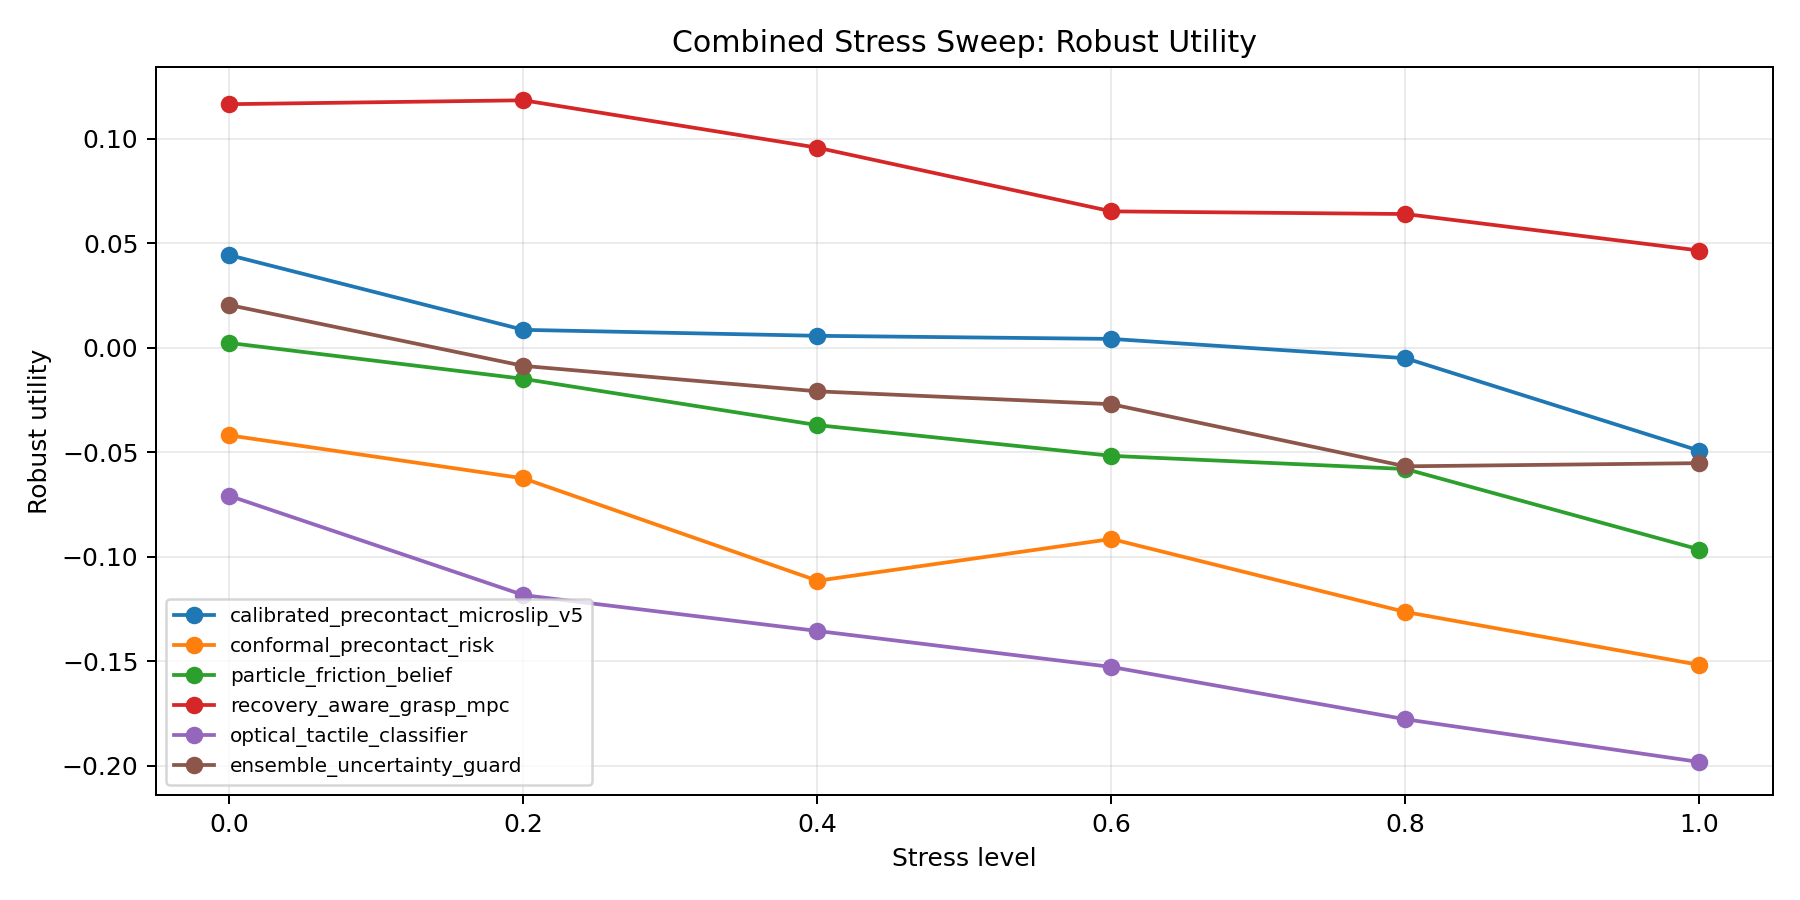
\includegraphics[width=\linewidth]{../figures/microslip_stress_sweep_v5.png}
\caption{Combined stress sweep. V5 is not the maximum-stress utility winner.}
\end{figure}

\section{Fixed-Risk Deployment}

\begin{longtable}{@{}ll llrr@{}}
\caption{Fixed-risk deployment budgets on hard splits. Budget 0.05 has zero accepted coverage for v5, so the deployment gate fails.}\\
\toprule
Split & Budget & Method & Metric & Mean & CI95 \\
\midrule
\endfirsthead
\toprule
Split & Budget & Method & Metric & Mean & CI95 \\
\midrule
\endhead
combined-hard & 0.0 & v5 & coverage & 0.000 & 0.000 \\
combined-hard & 0.0 & v5 & accepted\_success & 0.000 & 0.000 \\
combined-hard & 0.0 & v5 & accepted\_gross\_slip & 0.000 & 0.000 \\
combined-hard & 0.0 & v5 & accepted\_damage & 0.000 & 0.000 \\
combined-hard & 0.0 & conformal & coverage & 0.000 & 0.000 \\
combined-hard & 0.0 & conformal & accepted\_success & 0.000 & 0.000 \\
combined-hard & 0.0 & conformal & accepted\_gross\_slip & 0.000 & 0.000 \\
combined-hard & 0.0 & conformal & accepted\_damage & 0.000 & 0.000 \\
combined-hard & 0.0 & ensemble & coverage & 0.000 & 0.000 \\
combined-hard & 0.0 & ensemble & accepted\_success & 0.000 & 0.000 \\
combined-hard & 0.0 & ensemble & accepted\_gross\_slip & 0.000 & 0.000 \\
combined-hard & 0.0 & ensemble & accepted\_damage & 0.000 & 0.000 \\
combined-hard & 0.0 & mpc-grip & coverage & 0.000 & 0.000 \\
combined-hard & 0.0 & mpc-grip & accepted\_success & 0.000 & 0.000 \\
combined-hard & 0.0 & mpc-grip & accepted\_gross\_slip & 0.000 & 0.000 \\
combined-hard & 0.0 & mpc-grip & accepted\_damage & 0.000 & 0.000 \\
combined-hard & 0.0 & particle-friction & coverage & 0.000 & 0.000 \\
combined-hard & 0.0 & particle-friction & accepted\_success & 0.000 & 0.000 \\
combined-hard & 0.0 & particle-friction & accepted\_gross\_slip & 0.000 & 0.000 \\
combined-hard & 0.0 & particle-friction & accepted\_damage & 0.000 & 0.000 \\
combined-hard & 0.0 & recovery-mpc & coverage & 0.000 & 0.000 \\
combined-hard & 0.0 & recovery-mpc & accepted\_success & 0.000 & 0.000 \\
combined-hard & 0.0 & recovery-mpc & accepted\_gross\_slip & 0.000 & 0.000 \\
combined-hard & 0.0 & recovery-mpc & accepted\_damage & 0.000 & 0.000 \\
combined-hard & 0.05 & v5 & coverage & 0.000 & 0.000 \\
combined-hard & 0.05 & v5 & accepted\_success & 0.000 & 0.000 \\
combined-hard & 0.05 & v5 & accepted\_gross\_slip & 0.000 & 0.000 \\
combined-hard & 0.05 & v5 & accepted\_damage & 0.000 & 0.000 \\
combined-hard & 0.05 & conformal & coverage & 0.000 & 0.000 \\
combined-hard & 0.05 & conformal & accepted\_success & 0.000 & 0.000 \\
combined-hard & 0.05 & conformal & accepted\_gross\_slip & 0.000 & 0.000 \\
combined-hard & 0.05 & conformal & accepted\_damage & 0.000 & 0.000 \\
combined-hard & 0.05 & ensemble & coverage & 0.000 & 0.000 \\
combined-hard & 0.05 & ensemble & accepted\_success & 0.000 & 0.000 \\
combined-hard & 0.05 & ensemble & accepted\_gross\_slip & 0.000 & 0.000 \\
combined-hard & 0.05 & ensemble & accepted\_damage & 0.000 & 0.000 \\
combined-hard & 0.05 & mpc-grip & coverage & 0.000 & 0.000 \\
combined-hard & 0.05 & mpc-grip & accepted\_success & 0.000 & 0.000 \\
combined-hard & 0.05 & mpc-grip & accepted\_gross\_slip & 0.000 & 0.000 \\
combined-hard & 0.05 & mpc-grip & accepted\_damage & 0.000 & 0.000 \\
combined-hard & 0.05 & particle-friction & coverage & 0.000 & 0.000 \\
combined-hard & 0.05 & particle-friction & accepted\_success & 0.000 & 0.000 \\
combined-hard & 0.05 & particle-friction & accepted\_gross\_slip & 0.000 & 0.000 \\
combined-hard & 0.05 & particle-friction & accepted\_damage & 0.000 & 0.000 \\
combined-hard & 0.05 & recovery-mpc & coverage & 0.000 & 0.000 \\
combined-hard & 0.05 & recovery-mpc & accepted\_success & 0.000 & 0.000 \\
combined-hard & 0.05 & recovery-mpc & accepted\_gross\_slip & 0.000 & 0.000 \\
combined-hard & 0.05 & recovery-mpc & accepted\_damage & 0.000 & 0.000 \\
combined-hard & 0.1 & v5 & coverage & 0.000 & 0.000 \\
combined-hard & 0.1 & v5 & accepted\_success & 0.000 & 0.000 \\
combined-hard & 0.1 & v5 & accepted\_gross\_slip & 0.000 & 0.000 \\
combined-hard & 0.1 & v5 & accepted\_damage & 0.000 & 0.000 \\
combined-hard & 0.1 & conformal & coverage & 0.000 & 0.000 \\
combined-hard & 0.1 & conformal & accepted\_success & 0.000 & 0.000 \\
combined-hard & 0.1 & conformal & accepted\_gross\_slip & 0.000 & 0.000 \\
combined-hard & 0.1 & conformal & accepted\_damage & 0.000 & 0.000 \\
combined-hard & 0.1 & ensemble & coverage & 0.000 & 0.000 \\
combined-hard & 0.1 & ensemble & accepted\_success & 0.000 & 0.000 \\
combined-hard & 0.1 & ensemble & accepted\_gross\_slip & 0.000 & 0.000 \\
combined-hard & 0.1 & ensemble & accepted\_damage & 0.000 & 0.000 \\
combined-hard & 0.1 & mpc-grip & coverage & 0.000 & 0.000 \\
combined-hard & 0.1 & mpc-grip & accepted\_success & 0.000 & 0.000 \\
combined-hard & 0.1 & mpc-grip & accepted\_gross\_slip & 0.000 & 0.000 \\
combined-hard & 0.1 & mpc-grip & accepted\_damage & 0.000 & 0.000 \\
combined-hard & 0.1 & particle-friction & coverage & 0.000 & 0.000 \\
combined-hard & 0.1 & particle-friction & accepted\_success & 0.000 & 0.000 \\
combined-hard & 0.1 & particle-friction & accepted\_gross\_slip & 0.000 & 0.000 \\
combined-hard & 0.1 & particle-friction & accepted\_damage & 0.000 & 0.000 \\
combined-hard & 0.1 & recovery-mpc & coverage & 0.000 & 0.000 \\
combined-hard & 0.1 & recovery-mpc & accepted\_success & 0.000 & 0.000 \\
combined-hard & 0.1 & recovery-mpc & accepted\_gross\_slip & 0.000 & 0.000 \\
combined-hard & 0.1 & recovery-mpc & accepted\_damage & 0.000 & 0.000 \\
combined-hard & 0.15 & v5 & coverage & 0.000 & 0.000 \\
combined-hard & 0.15 & v5 & accepted\_success & 0.000 & 0.000 \\
combined-hard & 0.15 & v5 & accepted\_gross\_slip & 0.000 & 0.000 \\
combined-hard & 0.15 & v5 & accepted\_damage & 0.000 & 0.000 \\
combined-hard & 0.15 & conformal & coverage & 0.000 & 0.000 \\
combined-hard & 0.15 & conformal & accepted\_success & 0.000 & 0.000 \\
combined-hard & 0.15 & conformal & accepted\_gross\_slip & 0.000 & 0.000 \\
combined-hard & 0.15 & conformal & accepted\_damage & 0.000 & 0.000 \\
combined-hard & 0.15 & ensemble & coverage & 0.000 & 0.000 \\
combined-hard & 0.15 & ensemble & accepted\_success & 0.000 & 0.000 \\
combined-hard & 0.15 & ensemble & accepted\_gross\_slip & 0.000 & 0.000 \\
combined-hard & 0.15 & ensemble & accepted\_damage & 0.000 & 0.000 \\
combined-hard & 0.15 & mpc-grip & coverage & 0.000 & 0.000 \\
combined-hard & 0.15 & mpc-grip & accepted\_success & 0.000 & 0.000 \\
combined-hard & 0.15 & mpc-grip & accepted\_gross\_slip & 0.000 & 0.000 \\
combined-hard & 0.15 & mpc-grip & accepted\_damage & 0.000 & 0.000 \\
combined-hard & 0.15 & particle-friction & coverage & 0.000 & 0.000 \\
combined-hard & 0.15 & particle-friction & accepted\_success & 0.000 & 0.000 \\
combined-hard & 0.15 & particle-friction & accepted\_gross\_slip & 0.000 & 0.000 \\
combined-hard & 0.15 & particle-friction & accepted\_damage & 0.000 & 0.000 \\
combined-hard & 0.15 & recovery-mpc & coverage & 0.000 & 0.000 \\
combined-hard & 0.15 & recovery-mpc & accepted\_success & 0.000 & 0.000 \\
combined-hard & 0.15 & recovery-mpc & accepted\_gross\_slip & 0.000 & 0.000 \\
combined-hard & 0.15 & recovery-mpc & accepted\_damage & 0.000 & 0.000 \\
low-signal & 0.0 & v5 & coverage & 0.000 & 0.000 \\
low-signal & 0.0 & v5 & accepted\_success & 0.000 & 0.000 \\
low-signal & 0.0 & v5 & accepted\_gross\_slip & 0.000 & 0.000 \\
low-signal & 0.0 & v5 & accepted\_damage & 0.000 & 0.000 \\
low-signal & 0.0 & conformal & coverage & 0.000 & 0.000 \\
low-signal & 0.0 & conformal & accepted\_success & 0.000 & 0.000 \\
low-signal & 0.0 & conformal & accepted\_gross\_slip & 0.000 & 0.000 \\
low-signal & 0.0 & conformal & accepted\_damage & 0.000 & 0.000 \\
low-signal & 0.0 & ensemble & coverage & 0.000 & 0.000 \\
low-signal & 0.0 & ensemble & accepted\_success & 0.000 & 0.000 \\
low-signal & 0.0 & ensemble & accepted\_gross\_slip & 0.000 & 0.000 \\
low-signal & 0.0 & ensemble & accepted\_damage & 0.000 & 0.000 \\
low-signal & 0.0 & mpc-grip & coverage & 0.000 & 0.000 \\
low-signal & 0.0 & mpc-grip & accepted\_success & 0.000 & 0.000 \\
low-signal & 0.0 & mpc-grip & accepted\_gross\_slip & 0.000 & 0.000 \\
low-signal & 0.0 & mpc-grip & accepted\_damage & 0.000 & 0.000 \\
low-signal & 0.0 & particle-friction & coverage & 0.000 & 0.000 \\
low-signal & 0.0 & particle-friction & accepted\_success & 0.000 & 0.000 \\
low-signal & 0.0 & particle-friction & accepted\_gross\_slip & 0.000 & 0.000 \\
low-signal & 0.0 & particle-friction & accepted\_damage & 0.000 & 0.000 \\
low-signal & 0.0 & recovery-mpc & coverage & 0.000 & 0.000 \\
low-signal & 0.0 & recovery-mpc & accepted\_success & 0.000 & 0.000 \\
low-signal & 0.0 & recovery-mpc & accepted\_gross\_slip & 0.000 & 0.000 \\
low-signal & 0.0 & recovery-mpc & accepted\_damage & 0.000 & 0.000 \\
\bottomrule
\end{longtable}


\begin{figure}[t]
\centering
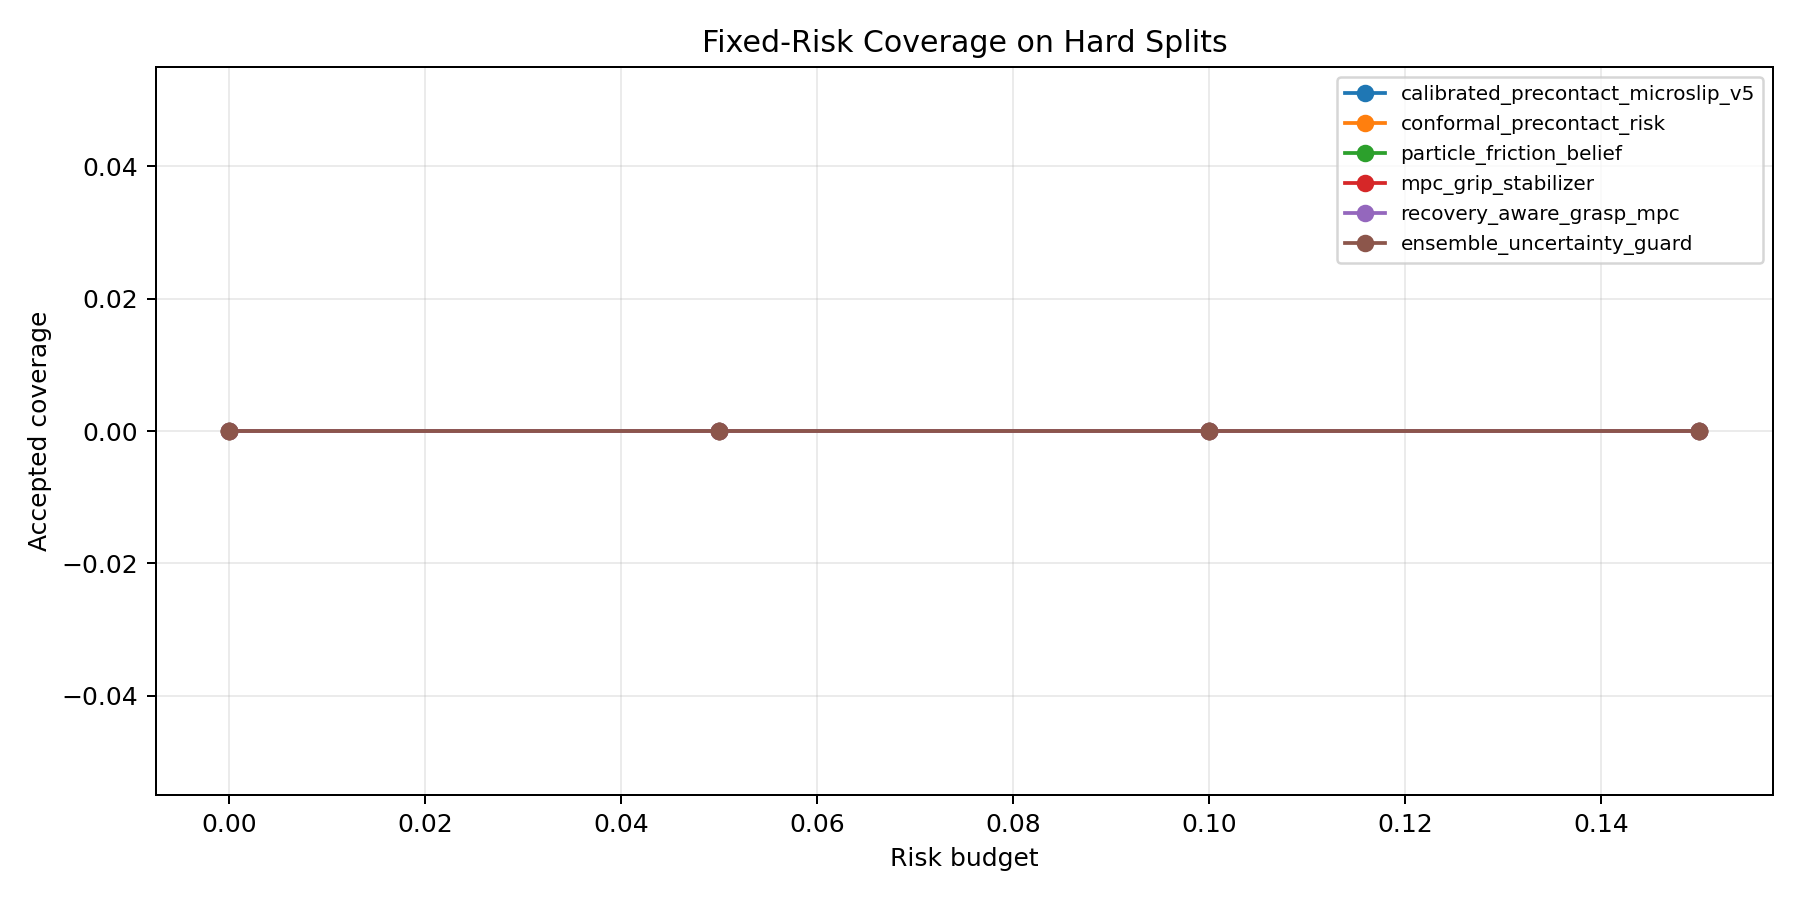
\includegraphics[width=\linewidth]{../figures/microslip_fixed_risk_v5.png}
\caption{Fixed-risk accepted coverage. Budget 0.05 has zero accepted coverage for v5 on hard deployment splits.}
\end{figure}

\section{Pareto and Negative Cases}
\begin{figure}[t]
\centering
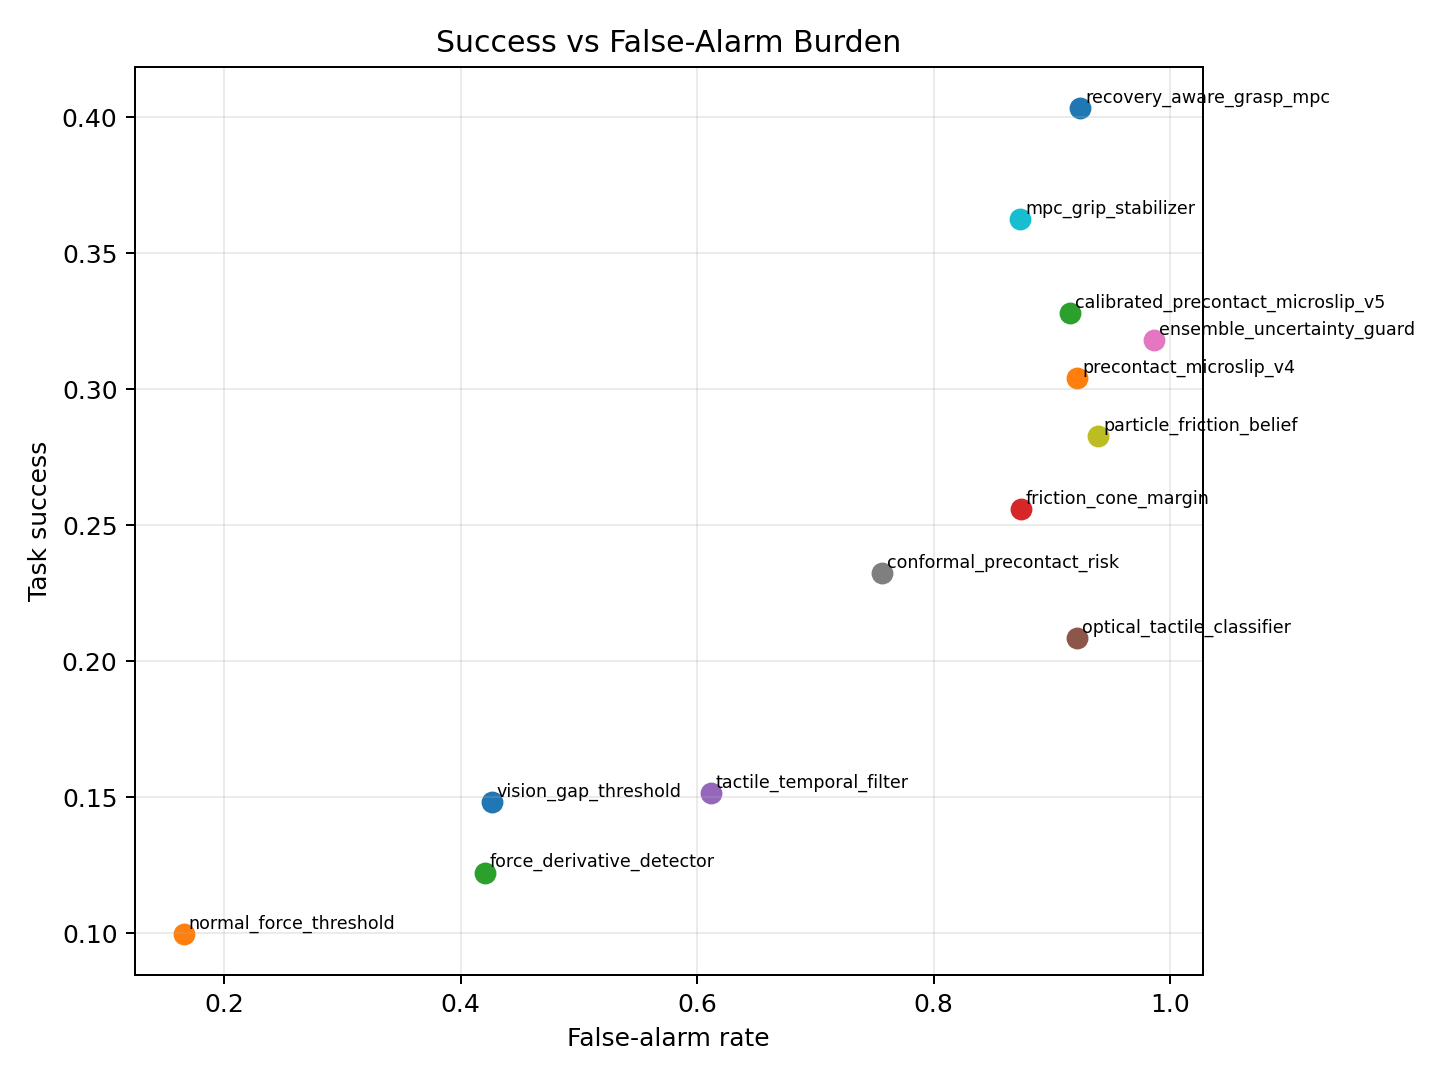
\includegraphics[width=0.85\linewidth]{../figures/microslip_pareto_v5.png}
\caption{Success versus false-alarm burden. V5 sits in a high-triggering region, while recovery-aware MPC gives better success/utility.}
\end{figure}


\begin{longtable}{@{}rlllrl@{}}
\caption{Negative cases selected from hard splits. These are not cherry-picked wins; they document where the proposed mechanism fails or over-triggers.}\\
\toprule
ID & Task & Split & Failure mode & v5 score & Baseline \\
\midrule
\endfirsthead
\toprule
ID & Task & Split & Failure mode & v5 score & Baseline \\
\midrule
\endhead
1 & compliant\_object\_lift & combined-hard & all\_non\_oracle\_fail & 0.691 & conformal\_precontact\_risk \\
2 & compliant\_object\_lift & combined-hard & false\_positive\_burden & 0.895 & conformal\_precontact\_risk \\
3 & compliant\_object\_lift & combined-hard & false\_positive\_burden & 0.864 & conformal\_precontact\_risk \\
4 & compliant\_object\_lift & combined-hard & all\_non\_oracle\_fail & 0.689 & conformal\_precontact\_risk \\
5 & compliant\_object\_lift & combined-hard & baseline\_recovers\_v5\_fails & 0.909 & particle\_friction\_belief \\
6 & compliant\_object\_lift & combined-hard & false\_positive\_burden & 1.000 & mpc\_grip\_stabilizer \\
7 & compliant\_object\_lift & combined-hard & baseline\_recovers\_v5\_fails & 1.000 & ensemble\_uncertainty\_guard \\
8 & compliant\_object\_lift & combined-hard & baseline\_recovers\_v5\_fails & 0.777 & conformal\_precontact\_risk \\
9 & compliant\_object\_lift & combined-hard & false\_positive\_burden & 0.680 & conformal\_precontact\_risk \\
10 & compliant\_object\_lift & combined-hard & all\_non\_oracle\_fail & 0.860 & recovery\_aware\_grasp\_mpc \\
11 & compliant\_object\_lift & combined-hard & all\_non\_oracle\_fail & 0.855 & conformal\_precontact\_risk \\
12 & compliant\_object\_lift & combined-hard & baseline\_recovers\_v5\_fails & 0.558 & recovery\_aware\_grasp\_mpc \\
13 & compliant\_object\_lift & combined-hard & false\_positive\_burden & 0.770 & conformal\_precontact\_risk \\
14 & compliant\_object\_lift & combined-hard & baseline\_recovers\_v5\_fails & 0.895 & particle\_friction\_belief \\
15 & compliant\_object\_lift & combined-hard & baseline\_recovers\_v5\_fails & 0.693 & recovery\_aware\_grasp\_mpc \\
16 & compliant\_object\_lift & combined-hard & all\_non\_oracle\_fail & 0.966 & conformal\_precontact\_risk \\
17 & compliant\_object\_lift & combined-hard & false\_positive\_burden & 1.000 & particle\_friction\_belief \\
18 & compliant\_object\_lift & combined-hard & baseline\_recovers\_v5\_fails & 0.823 & mpc\_grip\_stabilizer \\
19 & compliant\_object\_lift & combined-hard & false\_positive\_burden & 0.781 & recovery\_aware\_grasp\_mpc \\
20 & compliant\_object\_lift & combined-hard & baseline\_recovers\_v5\_fails & 0.903 & recovery\_aware\_grasp\_mpc \\
21 & compliant\_object\_lift & combined-hard & baseline\_recovers\_v5\_fails & 0.715 & particle\_friction\_belief \\
22 & compliant\_object\_lift & combined-hard & baseline\_recovers\_v5\_fails & 0.539 & recovery\_aware\_grasp\_mpc \\
23 & compliant\_object\_lift & combined-hard & baseline\_recovers\_v5\_fails & 0.854 & ensemble\_uncertainty\_guard \\
24 & compliant\_object\_lift & combined-hard & false\_positive\_burden & 0.812 & conformal\_precontact\_risk \\
\bottomrule
\end{longtable}


\section{What Improved Since v4}
The v5 method improves over \texttt{precontact\_microslip\_v4} on task success, gross-slip reduction, cost, chatter, recovery success, and robust utility. This matters: the rebuild did improve the method during development. The final protocol was then frozen, and the frozen result is still not enough. This is exactly why the paper should be archived rather than polished into a misleading submission.

\section{Scope and Limitations}
The largest limitation is external validity. There is no physical gripper, no real tactile dataset, no accepted high-fidelity tactile simulator, no trained controller checkpoint, and no independent reproduction. The benchmark is deterministic and useful for audit pressure, but not sufficient for a main-conference robotics claim.

\section{Terminal Recommendation}
The final recommendation is \textbf{KILL/ARCHIVE}. Revival requires real tactile or accepted high-fidelity evidence, calibrated fixed-risk deployment with nonzero coverage at strict budgets, and a method that beats particle friction belief and recovery-aware MPC without purchasing success through extreme false alarms.

\section{Hostile Citation Wall}
These citations are intentionally boxed by \texttt{hyperref} so clicking an in-text citation routes to the corresponding reference entry. \citep{r103390robotics8040085,r101186s40648024002733,r101109lra20223205768,r101109icra4663920229812186,r101299jsmermd2005682,r101017s0950268825100319} \citep{r1010800020754320222164628,r101109tim20233343795,r101089soro20200213,r101089soro20180172,r101109icra4663920229811832,r103390s17122762} \citep{r103390s19224925,r101007s4082001902887,r101126sciroboticsadq5046,r101109lra20243387111,r103390machines9060119,r103390s18020326} \citep{r101016jcej2023146279,r101109robot1996509203,r260611184v1,r101109tro20243502197,r103390app13063886,r101002rcs2491} \citep{r103390s19040966,r103389frobt20261735467,r101016jengfailanal2026110526,r101109icra55743202511127381,r101016jmeasurement2024114249,r101002adrr202500091} \citep{r101109lra20192930477,r101016jsna201907007,r101109icra57147202410611504,r101002rcs2325,r103389frobt2022913930,r103389frobt2021631371} \citep{r101016jisatra201812031,r101049csy270036,r1015607rss2022xviii070,r101109lra20213061378,r101109lra20253568616,r101109jsen20253547369} \citep{r220509430v2,r101017s0263574704001535,r101109robosoft55895202310121967,r103390machines10090720,r260609337v2,r260212532v1} \citep{r260223648v1,r101109icra55743202511127723,r101109lra20253604723,r101109lra20263662618,r1010800169186420181525075,r101007s41315022002600} \citep{r1011093516914388,r101108ir0120250033,r101109tro20203005547,r101007s1336902206763z,r1010800042311420252606345,r101007s41315025004948} \citep{r101109lra20253572817,r101109robot20041308042,r101016jprocs202310646,r101109robio20116181676,r191003973v1,r1054254275388182025ad28420} \citep{r101109robot20084543605,r101016jsna2025117179,r1011093mnano65639202511261038,r10114537942093794293,r101109newcas64648202511107072,r101299jsmermd200183} \citep{r101109iros60139202511245832,r101016jrobot2026105468,r101109icra20136630959,r101002adma202310145,r251223864v3,r230504660v1} \citep{r101109icra20198794087,r103390s20041050,r101109robio64047202410907710,r101109icma5203620219512714,r101109wrcsara5704020229903958,r101126sciadvadp6094} \citep{r103390agriculture14070996,r101002admt202100285,r107210jrsj41322,r101109icra20177989117,r10106314829919,r107210jrsj25970} \citep{r101109icsens20095398198,r101109tencon20084766846,r103390s23146547,r101109tmech20233276220,r101109jsen20223181128,r1036227techrxiv22145723} \citep{r103390mi15121513,r101109icarcv20188581233,r101126sciadvabd7795,r107210jrsj1991,r101109crc201749,r101109robio5416820219739442} \citep{r101016jjmpt201210010,r101109tmech20233264650,r101109sii20198700383,r103390app10186448,r101093bibbbac499,r103390s22114083} \citep{r101007s11071024099005,r101007s4054402308102,r101109access20192956882,r107210jrsj23337,r101002aisy202100047,r103390met10050685} \citep{r1036227techrxiv22145723v1,r101061ascecp194354870000899,r103390s23094433,r101109ascc20178287372,r101007978331928872714,r101126sciroboticsabm0608} \citep{r101038s41598019403141,r103390s23249640,r101109iros20126385899,r103390s23104786,r101109jsen20233262019,r1055677ijhrsss042025vol02i4} \citep{r103390machines11100955,r104172216896951000116,r101109devlrn20146982968,r107210jrsj13539,r101093ehjdhztad033,r103390lubricants11090356} \citep{r101002rob21833,r101002rob20179,r101109sii20178279340,r101038s4418202500055y,r101109cyber20188688163,r107210jrsj26767} \citep{r101109lra20203014634,r1011099754821,r260200514v2,r250302881v3,r250406156v2,r260222088v2} \citep{r260608555v1,r251013324v1,r260528412v1,r250116349v2,r250601941v4,r250916550v1} \citep{r101063100034396,r101109aim20188452704,r101142s0219843619400024,r103390s20174724,r101002rob22239,r101109ichr20051573549} \citep{r101541ieejjia5132,r1021203rs3rs7932705v1,r103390s26051473,r101371journalpone0335922} \citep{r101109iros60139202511245832,r101016jrobot2026105468,r101109icra20136630959,r101002adma202310145,r251223864v3,r230504660v1} \citep{r101109icra20198794087,r103390s20041050,r101109robio64047202410907710,r101109icma5203620219512714,r101109wrcsara5704020229903958,r101126sciadvadp6094} \citep{r103390agriculture14070996,r101002admt202100285,r107210jrsj41322,r101109icra20177989117,r10106314829919,r107210jrsj25970} \citep{r101109icsens20095398198,r101109tencon20084766846,r103390s23146547,r101109tmech20233276220,r101109jsen20223181128,r1036227techrxiv22145723} \citep{r103390mi15121513,r101109icarcv20188581233,r101126sciadvabd7795,r107210jrsj1991,r101109crc201749,r101109robio5416820219739442} \citep{r101016jjmpt201210010,r101109tmech20233264650,r101109sii20198700383,r103390app10186448,r101093bibbbac499,r103390s22114083} \citep{r101007s11071024099005,r101007s4054402308102,r101109access20192956882,r107210jrsj23337,r101002aisy202100047,r103390met10050685} \citep{r1036227techrxiv22145723v1,r101061ascecp194354870000899,r103390s23094433,r101109ascc20178287372,r101007978331928872714,r101126sciroboticsabm0608} \citep{r101038s41598019403141,r103390s23249640,r101109iros20126385899,r103390s23104786,r101109jsen20233262019,r1055677ijhrsss042025vol02i4} \citep{r103390machines11100955,r104172216896951000116,r101109devlrn20146982968,r107210jrsj13539,r101093ehjdhztad033,r103390lubricants11090356} \citep{r101002rob21833,r101002rob20179,r101109sii20178279340,r101038s4418202500055y,r101109cyber20188688163,r107210jrsj26767} \citep{r101109lra20203014634,r1011099754821,r260200514v2,r250302881v3,r250406156v2,r260222088v2} \citep{r260608555v1,r251013324v1,r260528412v1,r250116349v2,r250601941v4,r250916550v1} \citep{r101063100034396,r101109aim20188452704,r101142s0219843619400024,r103390s20174724,r101002rob22239,r101109ichr20051573549} \citep{r101541ieejjia5132,r1021203rs3rs7932705v1,r103390s26051473,r101371journalpone0335922}


\section{Raw Summary Extract}
\begin{tiny}
\begin{verbatim}
Paper 91 micro_slip_precontact_prediction v5 expanded audit
Terminal recommendation: KILL_ARCHIVE
ICLR main ready: no
Reason: expanded CPU-only micro-slip/precontact audit adds stronger optical-tactile,
conformal, particle-friction, MPC, recovery-aware, ablation, stress, and fixed-risk tests,
but no real robot or accepted high-fidelity tactile benchmark evidence exists.
Main rollout rows: 215040
Dataset summary rows: 15360
Main seed-metric rows: 1120
Main metric rows: 1456
Main pairwise rows: 1248
Hard aggregate seed rows: 140
Hard aggregate metric rows: 182
Hard aggregate pairwise rows: 156
Ablation rollout rows: 76800
Ablation seed rows: 100
Ablation metric rows: 130
Stress raw rows: 302400
Stress seed rows: 840
Stress metric rows: 1092
Fixed-risk raw rows: 69120
Fixed-risk seed rows: 480
Fixed-risk metric rows: 288
Fixed-risk pairwise rows: 240
Negative cases: 24

Frozen hard-aggregate gate:
best_ap_reference=particle_friction_belief
best_success_reference=recovery_aware_grasp_mpc
safest_reference=recovery_aware_grasp_mpc
lowest_damage_reference=recovery_aware_grasp_mpc
lowest_cost_reference=normal_force_threshold
best_calibration_reference=particle_friction_belief
lowest_false_alarm_reference=normal_force_threshold
best_utility_reference=recovery_aware_grasp_mpc
proposal_ap=0.80088
best_ap=0.80598
proposal_success=0.32799
best_success=0.40325
proposal_gross_slip=0.42383
safest_gross_slip=0.39844
proposal_damage=0.09401
lowest_damage=0.08359
proposal_false_alarm=0.91561
lowest_false_alarm=0.16578
proposal_cost=0.33957
lowest_cost=0.07896
proposal_ece=0.08042
best_ece=0.07205
proposal_utility=-0.02258
best_utility=0.06676
paired_ap_lower95=-0.01806
paired_success_lower95=-0.08393
paired_gross_slip_upper95=0.04221
paired_utility_lower95=-0.10436
main_gate=False
control_gate=False
safety_gate=False
calibration_gate=False
burden_gate=False
mechanism_gate=True
mechanism_best_ablation=full_precontact_microslip_v5
stress_gate=False
stress_dominated_by=recovery_aware_grasp_mpc
fixed_risk_gate=False
scope_gate=False
low_signal_high_risk_shift: v5_coverage=0.00000, v5_success=0.00000, v5_gross_slip=0.00000
combined_hard_shift: v5_coverage=0.00000, v5_success=0.00000, v5_gross_slip=0.00000

Hard aggregate metrics:
vision_gap_threshold ap=0.80227 auroc=0.55434 ece=0.20541 early=0.50557 false_alarm=0.42635
success=0.14831 gross=0.58047 damage=0.12240 cost=0.14470 utility=-0.22743
normal_force_threshold ap=0.78421 auroc=0.51271 ece=0.42070 early=0.18912
false_alarm=0.16578 success=0.09987 gross=0.64023 damage=0.13555 cost=0.07896
utility=-0.28574
force_derivative_detector ap=0.78129 auroc=0.51333 ece=0.28755 early=0.43278
false_alarm=0.42055 success=0.12240 gross=0.60898 damage=0.13425 cost=0.12172
utility=-0.26679
friction_cone_margin ap=0.79682 auroc=0.55072 ece=0.10276 early=0.91034 false_alarm=0.87410
success=0.25599 gross=0.46367 damage=0.10143 cost=0.28195 utility=-0.10182
tactile_temporal_filter ap=0.79296 auroc=0.53781 ece=0.18152 early=0.66922
false_alarm=0.61192 success=0.15156 gross=0.56706 damage=0.12604 cost=0.17178
utility=-0.23177
optical_tactile_classifier ap=0.79705 auroc=0.55053 ece=0.09320 early=0.95426
false_alarm=0.92127 success=0.20872 gross=0.50781 damage=0.11081 cost=0.27423
utility=-0.17434
ensemble_uncertainty_guard ap=0.79845 auroc=0.55426 ece=0.09426 early=0.99171
false_alarm=0.98631 success=0.31810 gross=0.41563 damage=0.08880 cost=0.45660
utility=-0.05561
conformal_precontact_risk ap=0.80258 auroc=0.56048 ece=0.07534 early=0.81950
false_alarm=0.75649 success=0.23242 gross=0.48359 damage=0.10599 cost=0.23184
utility=-0.11952
particle_friction_belief ap=0.80598 auroc=0.56041 ece=0.07205 early=0.96451
false_alarm=0.93913 success=0.28294 gross=0.45599 damage=0.09362 cost=0.28702
utility=-0.07117
mpc_grip_stabilizer ap=0.79680 auroc=0.54356 ece=0.10037 early=0.90812 false_alarm=0.87331
success=0.36250 gross=0.41523 damage=0.09232 cost=0.32733 utility=0.02490
recovery_aware_grasp_mpc ap=0.80004 auroc=0.54822 ece=0.10130 early=0.93688
false_alarm=0.92397 success=0.40325 gross=0.39844 damage=0.08359 cost=0.36671
utility=0.06676
precontact_microslip_v4 ap=0.80526 auroc=0.56131 ece=0.10484 early=0.94413
false_alarm=0.92158 success=0.30404 gross=0.43906 damage=0.09831 cost=0.41596
utility=-0.07360
calibrated_precontact_microslip_v5 ap=0.80088 auroc=0.55453 ece=0.08042 early=0.94663
false_alarm=0.91561 success=0.32799 gross=0.42383 damage=0.09401 cost=0.33957
utility=-0.02258
oracle_precontact_risk ap=0.85087 auroc=0.65211 ece=0.02345 early=0.99224
false_alarm=0.97270 success=0.60365 gross=0.23685 damage=0.04700 cost=0.31438
utility=0.37067

Key paired hard-aggregate differences:
calibrated_precontact_microslip_v5_minus_particle_friction_belief average_precision:
mean=-0.005094 ci95=0.012962 lower95=-0.018056 upper95=0.007868
calibrated_precontact_microslip_v5_minus_particle_friction_belief auroc: mean=-0.005884
ci95=0.023851 lower95=-0.029735 upper95=0.017967
calibrated_precontact_microslip_v5_minus_particle_friction_belief ece: mean=0.008373
ci95=0.013343 lower95=-0.004969 upper95=0.021716
calibrated_precontact_microslip_v5_minus_particle_friction_belief early_recall:
mean=-0.017877 ci95=0.005876 lower95=-0.023753 upper95=-0.012002
calibrated_precontact_microslip_v5_minus_particle_friction_belief false_alarm_rate:
mean=-0.023522 ci95=0.011604 lower95=-0.035126 upper95=-0.011919
calibrated_precontact_microslip_v5_minus_particle_friction_belief lead_time_margin:
mean=0.029876 ci95=0.000564 lower95=0.029312 upper95=0.030440
calibrated_precontact_microslip_v5_minus_particle_friction_belief task_success:
mean=0.045052 ci95=0.012903 lower95=0.032150 upper95=0.057955
calibrated_precontact_microslip_v5_minus_particle_friction_belief gross_slip: mean=-0.032162
ci95=0.018273 lower95=-0.050435 upper95=-0.013888
calibrated_precontact_microslip_v5_minus_particle_friction_belief damage_rate: mean=0.000391
ci95=0.005820 lower95=-0.005429 upper95=0.006211
calibrated_precontact_microslip_v5_minus_particle_friction_belief intervention_cost:
mean=0.052550 ci95=0.001348 lower95=0.051201 upper95=0.053898
calibrated_precontact_microslip_v5_minus_particle_friction_belief control_chatter:
mean=0.031356 ci95=0.000705 lower95=0.030651 upper95=0.032062
calibrated_precontact_microslip_v5_minus_particle_friction_belief recovery_success:
mean=0.043490 ci95=0.009227 lower95=0.034263 upper95=0.052716
calibrated_precontact_microslip_v5_minus_particle_friction_belief robust_utility:
mean=0.048585 ci95=0.015098 lower95=0.033487 upper95=0.063683
calibrated_precontact_microslip_v5_minus_recovery_aware_grasp_mpc average_precision:
mean=0.000849 ci95=0.013864 lower95=-0.013015 upper95=0.014713
calibrated_precontact_microslip_v5_minus_recovery_aware_grasp_mpc auroc: mean=0.006306
ci95=0.022926 lower95=-0.016619 upper95=0.029232
calibrated_precontact_microslip_v5_minus_recovery_aware_grasp_mpc ece: mean=-0.020881
ci95=0.014478 lower95=-0.035359 upper95=-0.006403
calibrated_precontact_microslip_v5_minus_recovery_aware_grasp_mpc early_recall:
mean=0.009749 ci95=0.004732 lower95=0.005017 upper95=0.014481
calibrated_precontact_microslip_v5_minus_recovery_aware_grasp_mpc false_alarm_rate:
mean=-0.008364 ci95=0.012499 lower95=-0.020863 upper95=0.004135
calibrated_precontact_microslip_v5_minus_recovery_aware_grasp_mpc lead_time_margin:
mean=0.009557 ci95=0.000719 lower95=0.008838 upper95=0.010276
calibrated_precontact_microslip_v5_minus_recovery_aware_grasp_mpc task_success:
mean=-0.075260 ci95=0.008674 lower95=-0.083934 upper95=-0.066587
calibrated_precontact_microslip_v5_minus_recovery_aware_grasp_mpc gross_slip: mean=0.025390
ci95=0.016823 lower95=0.008568 upper95=0.042213
calibrated_precontact_microslip_v5_minus_recovery_aware_grasp_mpc damage_rate: mean=0.010417
ci95=0.009327 lower95=0.001090 upper95=0.019743
calibrated_precontact_microslip_v5_minus_recovery_aware_grasp_mpc intervention_cost:
mean=-0.027146 ci95=0.001621 lower95=-0.028766 upper95=-0.025525
calibrated_precontact_microslip_v5_minus_recovery_aware_grasp_mpc control_chatter:
mean=0.026954 ci95=0.000688 lower95=0.026266 upper95=0.027642
calibrated_precontact_microslip_v5_minus_recovery_aware_grasp_mpc recovery_success:
mean=-0.051693 ci95=0.007581 lower95=-0.059273 upper95=-0.044112
calibrated_precontact_microslip_v5_minus_recovery_aware_grasp_mpc robust_utility:
mean=-0.089340 ci95=0.015019 lower95=-0.104359 upper95=-0.074322
calibrated_precontact_microslip_v5_minus_precontact_microslip_v4 average_precision:
mean=-0.004378 ci95=0.011636 lower95=-0.016014 upper95=0.007258
calibrated_precontact_microslip_v5_minus_precontact_microslip_v4 auroc: mean=-0.006787
ci95=0.019275 lower95=-0.026061 upper95=0.012488
calibrated_precontact_microslip_v5_minus_precontact_microslip_v4 ece: mean=-0.024414
ci95=0.008756 lower95=-0.033170 upper95=-0.015658
calibrated_precontact_microslip_v5_minus_precontact_microslip_v4 early_recall: mean=0.002497
ci95=0.006369 lower95=-0.003872 upper95=0.008866
calibrated_precontact_microslip_v5_minus_precontact_microslip_v4 false_alarm_rate:
mean=-0.005969 ci95=0.020909 lower95=-0.026878 upper95=0.014941
calibrated_precontact_microslip_v5_minus_precontact_microslip_v4 lead_time_margin:
mean=-0.010615 ci95=0.000911 lower95=-0.011526 upper95=-0.009704
calibrated_precontact_microslip_v5_minus_precontact_microslip_v4 task_success: mean=0.023958
ci95=0.010385 lower95=0.013573 upper95=0.034344
calibrated_precontact_microslip_v5_minus_precontact_microslip_v4 gross_slip: mean=-0.015234
ci95=0.014705 lower95=-0.029939 upper95=-0.000529
calibrated_precontact_microslip_v5_minus_precontact_microslip_v4 damage_rate: mean=-0.004297
ci95=0.008849 lower95=-0.013146 upper95=0.004552
calibrated_precontact_microslip_v5_minus_precontact_microslip_v4 intervention_cost:
mean=-0.076388 ci95=0.002690 lower95=-0.079078 upper95=-0.073698
calibrated_precontact_microslip_v5_minus_precontact_microslip_v4 control_chatter:
mean=-0.040083 ci95=0.001184 lower95=-0.041267 upper95=-0.038899
calibrated_precontact_microslip_v5_minus_precontact_microslip_v4 recovery_success:
mean=0.021484 ci95=0.008180 lower95=0.013305 upper95=0.029664
calibrated_precontact_microslip_v5_minus_precontact_microslip_v4 robust_utility:
mean=0.051021 ci95=0.015200 lower95=0.035822 upper95=0.066221

Ablation utility:
full_precontact_microslip_v5 ap=0.80371 success=0.33307 gross=0.42357 false_alarm=0.90523
utility=-0.01732
minus_precontact_shear ap=0.79075 success=0.20352 gross=0.52865 false_alarm=0.75554
utility=-0.17265
minus_friction_prior ap=0.80111 success=0.26810 gross=0.46719 false_alarm=0.81485
utility=-0.08976
minus_compliance_model ap=0.80275 success=0.28203 gross=0.44557 false_alarm=0.90170
utility=-0.07413
minus_latency_margin ap=0.79891 success=0.28425 gross=0.44675 false_alarm=0.95234
utility=-0.07126
minus_calibration_layer ap=0.80064 success=0.32396 gross=0.42773 false_alarm=0.97305
utility=-0.06229
minus_visual_gap ap=0.80300 success=0.28047 gross=0.45729 false_alarm=0.91670
utility=-0.08449
minus_recovery_model ap=0.80642 success=0.26276 gross=0.45482 false_alarm=0.90870
utility=-0.10285
vision_only_precontact ap=0.79340 success=0.15221 gross=0.57148 false_alarm=0.44939
utility=-0.22157
force_only_precontact ap=0.78226 success=0.12838 gross=0.60521 false_alarm=0.42264
utility=-0.25716

Maximum combined stress:
vision_gap_threshold ap=0.83843 success=0.13972 gross=0.61667 utility=-0.25349
normal_force_threshold ap=0.82220 success=0.08944 gross=0.66250 utility=-0.30877
force_derivative_detector ap=0.81587 success=0.10694 gross=0.63389 utility=-0.29544
friction_cone_margin ap=0.83834 success=0.25833 gross=0.49861 utility=-0.11442
tactile_temporal_filter ap=0.82602 success=0.12028 gross=0.60556 utility=-0.28301
optical_tactile_classifier ap=0.82933 success=0.18722 gross=0.51972 utility=-0.19831
ensemble_uncertainty_guard ap=0.82159 success=0.32361 gross=0.43750 utility=-0.05528
conformal_precontact_risk ap=0.81618 success=0.22222 gross=0.52500 utility=-0.15185
particle_friction_belief ap=0.82243 success=0.27139 gross=0.48972 utility=-0.09663
mpc_grip_stabilizer ap=0.81237 success=0.35361 gross=0.41000 utility=0.01945
recovery_aware_grasp_mpc ap=0.82341 success=0.38417 gross=0.40305 utility=0.04646
precontact_microslip_v4 ap=0.83284 success=0.28333 gross=0.45389 utility=-0.09664
calibrated_precontact_microslip_v5 ap=0.82039 success=0.30861 gross=0.44889 utility=-0.04937

Fixed-risk budget 0.05:
low_signal_high_risk_shift calibrated_precontact_microslip_v5 coverage=0.00000
accepted_success=0.00000 accepted_gross_slip=0.00000 accepted_damage=0.00000
low_signal_high_risk_shift conformal_precontact_risk coverage=0.00000
accepted_success=0.00000 accepted_gross_slip=0.00000 accepted_damage=0.00000
low_signal_high_risk_shift particle_friction_belief coverage=0.00000
accepted_success=0.00000 accepted_gross_slip=0.00000 accepted_damage=0.00000
low_signal_high_risk_shift mpc_grip_stabilizer coverage=0.00000 accepted_success=0.00000
accepted_gross_slip=0.00000 accepted_damage=0.00000
low_signal_high_risk_shift recovery_aware_grasp_mpc coverage=0.00000
accepted_success=0.00000 accepted_gross_slip=0.00000 accepted_damage=0.00000
low_signal_high_risk_shift ensemble_uncertainty_guard coverage=0.00000
accepted_success=0.00000 accepted_gross_slip=0.00000 accepted_damage=0.00000
combined_hard_shift calibrated_precontact_microslip_v5 coverage=0.00000
accepted_success=0.00000 accepted_gross_slip=0.00000 accepted_damage=0.00000
combined_hard_shift conformal_precontact_risk coverage=0.00000 accepted_success=0.00000
accepted_gross_slip=0.00000 accepted_damage=0.00000
combined_hard_shift particle_friction_belief coverage=0.00000 accepted_success=0.00000
accepted_gross_slip=0.00000 accepted_damage=0.00000
combined_hard_shift mpc_grip_stabilizer coverage=0.00000 accepted_success=0.00000
accepted_gross_slip=0.00000 accepted_damage=0.00000
combined_hard_shift recovery_aware_grasp_mpc coverage=0.00000 accepted_success=0.00000
accepted_gross_slip=0.00000 accepted_damage=0.00000
combined_hard_shift ensemble_uncertainty_guard coverage=0.00000 accepted_success=0.00000
accepted_gross_slip=0.00000 accepted_damage=0.00000

\end{verbatim}
\end{tiny}


\bibliographystyle{iclr2026_conference}
\bibliography{references}

\end{document}
